\documentclass[10pt,A5]{article}	
\usepackage[utf8]{inputenc}		
\usepackage{xstring, xifthen}
\usepackage[default]{raleway}
\renewcommand*\familydefault{\sfdefault} 	
\usepackage[T1]{fontenc}
\usepackage{moresize}
\usepackage{fontawesome}
\newcommand{\vcenteredinclude}[1]{\begingroup
\setbox0=\hbox{\includegraphics{#1}}%
\parbox{\wd0}{\box0}\endgroup}
\newcommand*{\vcenteredhbox}[1]{\begingroup
\setbox0=\hbox{#1}\parbox{\wd0}{\box0}\endgroup}
\newcommand{\icon}[3] { 							
	\makebox(#2, #2){\textcolor{maincol}{\csname fa#1\endcsname}}
}	
\newcommand{\icontext}[4]{ 						
	\vcenteredhbox{\icon{#1}{#2}{#3}}  \hspace{7pt}  \parbox{0.9\mpwidth}{\textcolor{#4}{#3}}
}
\newcommand{\iconhref}[5]{ 						
    \vcenteredhbox{\icon{#1}{#2}{#5}}  \hspace{2pt} \href{#4}{\textcolor{#5}{#3}}
}
\newcommand{\iconemail}[5]{ 						
    \vcenteredhbox{\icon{#1}{#2}{#5}}  \hspace{2pt} \href{mailto:#4}{\textcolor{#5}{#3}}
}
\usepackage{paracol}
\usepackage[a4paper]{geometry}
\geometry{top=0.5cm, bottom=0.5cm, left=0.5cm, right=0.5cm}
\usepackage{fancyhdr}
\pagestyle{empty}
\setlength{\parindent}{0mm}
\usepackage{array}
\newcolumntype{x}[1]{%
{\raggedleft\hspace{0pt}}p{#1}}%
\usepackage{graphicx}
\usepackage{tikz}				
\usetikzlibrary{shapes, backgrounds,mindmap, trees}
\usepackage{transparent}
\usepackage{color}
\definecolor{maincol}{RGB}{ 225, 0, 0 }
\definecolor{darkcol}{RGB}{ 70, 70, 70 }
\definecolor{lightcol}{RGB}{245,245,245}
\usepackage[hidelinks]{hyperref}
\newcommand{\mpwidth}{\linewidth-\fboxsep-\fboxsep}
\newcommand{\cvlist}[1] {
	\begin{itemize}{#1}\end{itemize}
}
\newcommand{\cvtext}[1] {
	\begin{tabular*}{1\mpwidth}{p{0.98\mpwidth}}
		\parbox{1\mpwidth}{#1}
	\end{tabular*}
}
\newcommand{\cvsection}[1] {
	\vspace{5pt}
	\cvtext{
		\textbf{\LARGE{\textcolor{darkcol}{\uppercase{#1}}}}\\[-6pt]
		\textcolor{maincol}{ \rule{0.1\textwidth}{3pt} } \\
	}
}

\newcommand{\cvskill}[3] {
	\begin{tabular*}{1\mpwidth}{p{0.72\mpwidth}  r}
 		\textcolor{black}{\textbf{#1}} & \textcolor{maincol}{#2}\\
	\end{tabular*}
	
	\hspace{5pt}
	\begin{tikzpicture}[scale=1,rounded corners=2pt,very thin]
		\fill [lightcol] (0,0) rectangle (1\mpwidth, 0.15);
		\fill [maincol] (0,0) rectangle (#3\mpwidth, 0.15);
  	\end{tikzpicture}
}

\newcommand{\cvevent}[5] {
	\parbox{\mpwidth}{
		\begin{tabular*}{1\mpwidth}{p{0.72\mpwidth}  r}
	 		\textcolor{black}{\textbf{#2}} & \colorbox{maincol}{\makebox[0.25\mpwidth]{\textcolor{white}{#1}}} \\
			\textcolor{maincol}{\textbf{#3}} & \\
		\end{tabular*}\\[4pt]
	
		\ifthenelse{\isempty{#4}}{}{
			\cvtext{#4}\\
		}
	}

	\ifthenelse{\isempty{#5}}{}{
		\vspace{2pt}
		{#5}
	}
}

\newcommand{\cvmetaevent}[4] {
	\textcolor{maincol} {\cvtext{\textbf{\begin{flushleft}#1\end{flushleft}}}}
	
	\ifthenelse{\isempty{#2}}{}{
		\textcolor{darkcol} {\cvtext{\begin{flushleft}#2\end{flushleft}}}}
	
	\ifthenelse{\isempty{#3}}{}{
		\textcolor{black} {\cvtext{\begin{flushleft}#3\end{flushleft}}}}
	
	\ifthenelse{\isempty{#4}}{}{
		\cvlist{#4}}
}

\newcommand{\cvqrcode}[1] {
	\begin{center}
		\includegraphics[width={#1}\mpwidth]{qrcode}
	\end{center}
}

\begin{document}
\columnratio{0.31}
\setlength{\columnsep}{2.2em}
\setlength{\columnseprule}{2pt}
\colseprulecolor{lightcol}
\begin{paracol}{2}
\begin{leftcolumn}

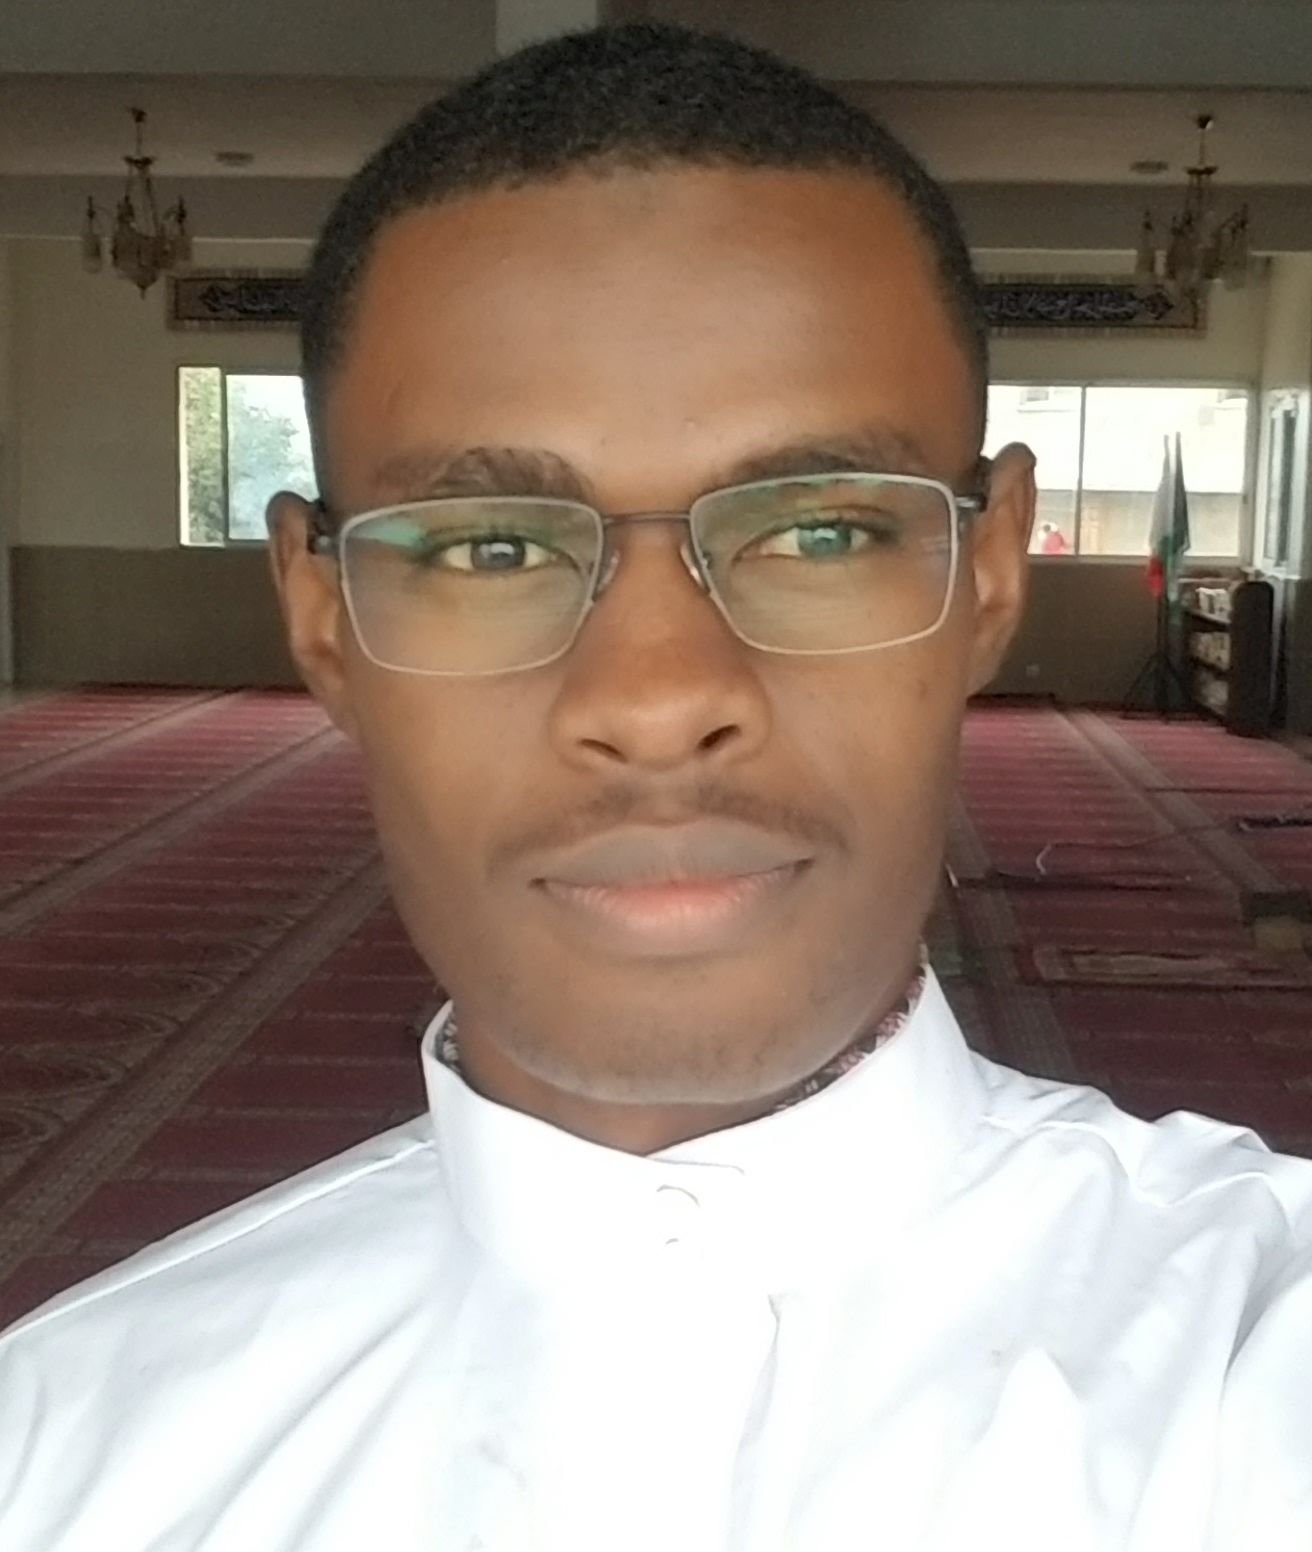
\includegraphics[width=\linewidth]{untitled.png}	

\cvsection{COMP\' ETENCES}

\cvskill{Node JS} {85 \%} {0.85} \\[-7pt]

\cvskill{Laravel} {75 \%} {0.75} \\[-7pt]

\cvskill{React JS} {70 \% } {0.70} \\[-7pt]

\cvskill{Angular} {65 \%} {0.65} \\[-7pt]

\cvskill{ASP.Net} {65 \%} {0.65} \\[-7pt]

\cvsection{HOBBIES}

\cvskill{BasketBall \& Musculation} {Sport} {1} \\[-7pt]

\cvskill{Livre Scientifique \& Réportage} {Loisir} {1} \\[-7pt]

\cvsection{CONTACTS}
	
\icontext{MapMarker}{12}{III F 25 Bis Antananarive\\ Antohomadinika Avaratra}{black}\\[6pt]
\icontext{MobilePhone}{12}{+261 38 72 657 05 }{black}\\[6pt]
\iconemail{Envelope}{12}{raharison.tsidiany@esti.mg}{raharison.tsidiany@esti.mg}{black}\\[6pt]
\verb| |\faLinkedinSquare \quad Raharison Muriel TSIDIANY \\[6pt]
\verb| |\faTwitter \quad @MurielTsidany \\[6pt]
\verb| |\faGithubSquare \quad https://github.com/DevSuccess \\[6pt]

\cvqrcode{0.45}

\end{leftcolumn}
\begin{rightcolumn}

\fcolorbox{white}{darkcol}{\begin{minipage}[c][3.5cm][c]{1\mpwidth}
	\begin {center}
		\HUGE{ \textbf{ \textcolor{white}{ \uppercase{ TSIDIANY Raharison Muriel } } } } \\[-24pt]
		\textcolor{white}{ \rule{0.1\textwidth}{1.25pt} } \\[4pt]
		\large{ \textcolor{white} {Développeur Informatique} }
	\end {center}
\end{minipage}} \\[12pt]
\vspace{-12pt}

\cvsection{PROFIL}

\cvtext{Je suis un \textbf{développeur web} passionné de 22 ans ayant acquis une solide expérience en travaillant en tant que freelance sur plusieurs projets. En tant qu'\textbf{autodidacte motivé}, je suis capable de travailler de manière \textbf{autonome} et je suis constamment à la recherche de nouveaux projets pour continuer à développer mes compétences. Je suis particulièrement compétent dans les domaines de la programmation \textbf{front-end} et \textbf{back-end}, ainsi que dans l'utilisation de diverses technologies de développement web.\\}

\cvsection{PARCOURS SCOLAIRE}

\cvevent
{Février 2020 - Now}
{\'Etudes Universitaire}
{A propos}
{J'ai suivi des parcours concernant l'informatique dans les universités qui sont spécialisées dans ce domaine, telles que :}
{\cvlist{
		\item \textbf{ESTI :} Licence 1 et 2 en Développement Informatique.
		\item \textbf{ESMIA :} Licence 1 en Informatique Risque et Décision. (2020-2021)
}}

\cvsection{EXP\' ERIENCES}

\cvevent
{Janvier - Avril 2023}
{Stage à l'entreprise Accès Banque Madagascar}
{En Développement Web}
{Au sein de ABM, j’ai acquis une expérience de stage significative en développement web, avec une focalisation particulière sur les technologies suivantes  :}
{\cvlist{
		\item \textbf{Front-End :} Angular
		\item \textbf{Back-End :} ASP.Net, Fluent NHibernate et NHibernate
}}

\cvevent
	{Juin 2021 - Now}
	{Président et Fondateur de l'Association ITDevSuccess}
	{Une Association de jeune passioner de l'informatique}
	{Cette association regroupe une poignée de jeunes passionnés de l’informatique qui sont soit étudiants dans des universités, soit des professionnels travaillant dans le domaine de l'IT:}
	{\cvlist{
		\item \textbf{Université :} ESTI, ESMIA, ITU, ENI, UPH. 
		\item \textbf{Entreprise :} Tech AIDMadagascar
	}}


\cvsection{T\'ECHNOLOGIES}

\cvtext{Les différentes téchnologies avec ou hors cursus Universitaire maîtrisés : 
\\}
{\cvlist{
		\item Les Technologies \textbf{Web} et leurs différentes notions : 
			\cvlist{
				\item \textbf{FrontEnd :} HTML5, CSS3, BootStrap, React JS, Angular   
				\item \textbf{BackEnd :} NodeJS, Express JS, Laravel, ASP.Net
				\item \textbf{DataBase :} MongoDb, MySQL, SQLite
				\item \textbf{Design Patterns :} MVC, Pattern Singleton, \dots
			}
		\item Le langague \textbf{Python} et ses Framework et librairies (Matplotbil, numpy et PyQt5).
		\begin{center}
			\textbf{À Jour le \textit{03 Mai 2023}}
		\end{center}	
	}}

\mbox{}
\mbox{}
\mbox{}
\mbox{}
\end{rightcolumn}
\end{paracol}
\end{document}